\documentclass[12pt]{article}
%%% Algorithm %%%
\usepackage{algorithm,algorithmicx,algpseudocode}

%%%
\usepackage{color,bold-extra,mathrsfs,float,bbm}
\usepackage[tableposition=t]{caption}
\captionsetup{textfont={small,it},labelfont={small, sc}}
\captionsetup[figure]{name=Fig.}
\usepackage{comment,graphics,aliascnt}
\usepackage[dvipsnames]{xcolor}
\usepackage[colorlinks=true,
linkcolor=red,
urlcolor=red,
citecolor=blue,
bookmarksopen=true,
pageanchor=false]{hyperref}
\usepackage[hyperpageref]{backref}
\renewcommand*{\backref}[1]{}% for backref < 1.33 necessary
\renewcommand*{\backrefalt}[4]{%
\ifcase #1 %
No citations.%
\or
(Cited on page #2.)
\else
(Cited on pages #2.)
\fi
}
\usepackage{enumerate,amsmath,amsfonts,amssymb,comment,mathtools}
\usepackage{amsthm}

%%

% \usepackage{lastpage}
\usepackage{fancyhdr}
\pagestyle{fancy}
\lhead{Polar Decomposition Project}
\rhead{\leftmark}
% \fancyfoot[C]{Page~\thepage~of~\pageref*{LastPage}}
\setlength{\headheight}{14.49998pt}

%% Fonts %%

\usepackage[T1]{fontenc}
\DeclareFontFamily{OT1}{rsfs}{}
\DeclareFontShape{OT1}{rsfs}{n}{it}{<-> rsfs10}{}
\DeclareMathAlphabet{\mathscr}{OT1}{rsfs}{n}{it}
\usepackage{lmodern} \normalfont %to load T1lmr.fd
\DeclareFontShape{T1}{lmr}{bx}{sc} { <-> ssub * cmr/bx/sc }{}
\usefont{T1}{qzc}{m}{it}
\usepackage{eucal}

% \usepackage[lucidascale=false]{lucimatx}
% \AtBeginDocument{
%   \DeclareSymbolFont{AMSb}{U}{msb}{m}{n}
%   \DeclareSymbolFontAlphabet{\mathbb}{AMSb}}

%% MATLAB Code %%% From Dr. Chris Johnson
\usepackage{listings}
\definecolor{codegreen}{rgb}{0,0.6,0}
\definecolor{codegray}{rgb}{0.5,0.5,0.5}
\definecolor{codepurple}{rgb}{0.58,0,0.82}
\definecolor{mygreen}{RGB}{28,172,0}
\definecolor{mylilas}{RGB}{170,55,241}
\definecolor{backcolour}{rgb}{0.95,0.95,1.92}
\lstdefinestyle{mystyle}{
	language=matlab,
  commentstyle=\color{codegreen},
  keywordstyle=\color{blue},
  numberstyle=\tiny\color{codegray},
  stringstyle=\color{codepurple},
  basicstyle=\linespread{0.9}\ttfamily\footnotesize,
  breakatwhitespace=false,
  breaklines=true,
  captionpos=b,
  keepspaces=true,
  numbers=left,
  numbersep=5pt,
  showspaces=false,
  showstringspaces=false,
  showtabs=false,
  tabsize=2,
  aboveskip=\medskipamount,
  frame=single,
}
\lstset{style=mystyle}
% \inline is a custom macro
\def\inline{\lstinline[basicstyle=\upshape\ttfamily\small]}

\DeclareCaptionLabelSeparator{separation}{:\quad}

%% Some definitions %%
\DeclarePairedDelimiter\ceil{\lceil}{\rceil}
\DeclarePairedDelimiter\floor{\lfloor}{\rfloor}
\usepackage{bm}
\DeclarePairedDelimiter\abs{\lvert}{\rvert}
\DeclarePairedDelimiter\inner{\langle}{\rangle}
% real and imaginary
\renewcommand{\Re}[1]{\mathfrak{Re}\left\{{#1}\right\}}
\renewcommand{\Im}[1]{\mathfrak{Im}\left\{{#1}\right\}}

\newcommand{\intii}{\int_{-\infty}^{\infty}}

%% Theorems %%
\newtheorem{theorem}{Theorem}[section]
\newtheorem{lemma}[theorem]{Lemma}
\newtheorem{proposition}[theorem]{Proposition}
\newtheorem{assumption}[theorem]{Assumption}
\newtheorem{corollary}[theorem]{Corollary}

\theoremstyle{definition}
\newtheorem{definition}[theorem]{Definition}
\newtheorem{remark}[theorem]{Remark}
\newtheorem{example}[theorem]{Example}
\newtheorem*{note}{Note}
\newtheorem*{question}{Question}
\newtheorem*{recall}{Recall}
\newtheorem{exercise}[theorem]{Exercise}

\numberwithin{equation}{section}

%% mathbb %%
\newcommand{\N}{\mathbb{N}} % natural numbers 
\newcommand{\Z}{\mathbb{Z}} % integers 
\newcommand{\Q}{\mathbb{Q}} % rationals
\newcommand{\R}{\mathbb{R}} % reals
\newcommand{\C}{\mathbb{C}} % complex
\newcommand{\F}{\mathbb{F}}

%% Probability %%
\renewcommand{\P}{\mathbb{P}} % probability
\DeclareMathOperator{\E}{\mathbb{E}} % expectation
\DeclareMathOperator{\V}{\mathbf{Var}} % variance

%% matrix and vectors %%
\newcommand{\n}{^n}
\newcommand{\Rn}{\R^n}
\newcommand{\mn}{^{m\times n}}
\newcommand{\nn}{^{n\times n}}
\renewcommand{\ij}{_{ij}}
\newcommand{\tp}{^T} 
\newcommand{\ctp}{^*}
\newcommand{\inv}{^{-1}}
\newcommand{\diag}{\mathrm{diag}}
\newcommand{\rank}{\mathrm{rank}}
\newcommand{\tr}{\mathrm{trace}}
\renewcommand{\det}{\mathrm{det}}
\newcommand{\range}{Range}
\renewcommand{\dim}{dim}
\renewcommand{\span}{span}
\newcommand{\eref}[1]{\eqref{#1}}

%% Symbols %%
\newcommand{\mat}{MATLAB}
\newcommand{\wh}{\widehat}
\newcommand{\wt}{\widetilde}
\newcommand{\wb}{\overline}
\newcommand{\grad}{\nabla}
\renewcommand{\div}{\nabla\cdot}
\newcommand{\curl}{\nabla\times}
\newcommand{\lap}{\varDelta}
\newcommand{\dd}{\mathrm{d}}
\newcommand{\pp}{\partial}
\def\eu{\mathrm{e}} % euler's constant
\def\im{\mathrm{i}} % imaginary unit

%%%% Greek Letters %%%%
\renewcommand{\a}{\alpha}
\newcommand{\lam}{\lam}
\renewcommand{\L}{\Lambda}
\newcommand{\vL}{\varLambda}
\renewcommand{\b}{\beta}
\newcommand{\p}{\phi}
\newcommand{\x}{\xi}
\newcommand{\G}{\Gamma}
\newcommand{\vG}{\varGamma}
\renewcommand{\O}{\Omega}
\newcommand{\vO}{\varOmega}
\renewcommand{\o}{\omega}
\newcommand{\e}{\epsilon}

% MSc project macros%
\def\ycite[#1#2#3#4#5]#6{\cite[$\mit{#1#2#3#4}$#5]{#6}}
\newcommand{\iter}[1]{^{(#1)}} % iteration
\newcommand{\norm}[1]{\|{#1}\|_2} % 2-norm
\newcommand{\sign}[1]{\mathrm{sign}\left({#1}\right)}
\renewcommand{\Sigma}{\varSigma} % skew sigma
\newcommand{\off}{\mathsf{off}} % off operator
\newcommand{\gnorm}[1]{\|{#1}\|}
\newcommand{\inorm}[1]{\|{#1}\|_{\infty}}

%% Defined Proof Evironment %%

\def\proof{\par{\bf Proof}. \ignorespaces}
\def\qedsymbol{\vbox{\hrule\hbox{%
                     \vrule height1.3ex\hskip0.8ex\vrule}\hrule}}
\def\endproof{\qquad\qedsymbol\medskip\par}

\title{Project : Computing the Polar Decomposition}
\author{Zhengbo Zhou%
    \thanks{%
        Department of Mathematics,
        University of Manchester,
        Manchester, M13 9PL, England
        (\texttt{zhengbo.zhou@postgrad.manchester.ac.uk}).
    }
}
\date{September 22, 2022}

\begin{document}
\maketitle


\section{Preliminaries}\label{sec:norms-svd}

\subsection{Vector Norms} \label{subsec:vector-norms}

Before introducing the matrix norm, a brief illustration of the vector norm is necessary.

\begin{definition}
  [Vector Norm] \label{def:vector-norm}
  A vector norm on $\C^n$ is a function $\gnorm{\cdot} : \C^n \to \R$  that  satisfies the  properties
  \begin{enumerate}
    \item $\gnorm{x} \geq 0$ for all $x\in\C\n$,
    \item $\gnorm{x} = 0$ if and only if $x = 0$,
    \item $\gnorm{\lambda x} = \abs{\lambda} \gnorm{x}$ for all $\lambda \in \C$ and $x \in \C^n$,
    \item $\gnorm{x + y} \leq \gnorm{x} + \gnorm{y}$ for all $x,y\in \C^n$.
  \end{enumerate}
\end{definition}

\begin{example}
    For $x\in\C^n$, 
    \begin{equation}\notag
        \begin{aligned}
            \text{1-norm : }& \gnorm{x}_1 = \sum_{i = 1}^n \abs{x_i},\\
            \text{2-norm (Euclidean Norm) : }& \tnorm{x} = \left(\sum_{i = 1}^n \abs{x_i}^2\right)^{1/2} = \sqrt{x\ctp x},\\
            \text{$\infty$-norm : } & \gnorm{x}_{\infty} = \max_{1\leq i \leq n} \abs{x_i}.
        \end{aligned}
    \end{equation}
    
    These are all special cases of the $p$-norm,
    \begin{equation}\label{eq:vector-p-norm}
        \gnorm{x}_p = \left(\sum_{i = 1}^n \abs{x_i}^p\right)^{1/p},\quad q \geq 1.
    \end{equation}
\end{example}

\subsection{Matrix Norms} \label{subsec:matrix-norms}
\begin{definition}
    [Matrix Norms]
    A matrix norm is a function $\gnorm{\cdot}:\C\mn \to \R$ that satisfies the analogues of the four properties in the Definition~\ref{def:vector-norm}.
\end{definition}

\begin{example}
    [Frobenius norm]
    For $A\in\C\mn$, the Frobenius norm is defined as
    \begin{equation}
        \notag
        \gnorm{A}_F = \left(\sum_{i = 1}^m \sum_{j = 1}^n \abs{a_{ij}}^2\right)^{1/2} = \left(\tr(A\ctp A)\right)^{1/2}.
    \end{equation}
\end{example}

\begin{example}
    [Subordinate matrix norm]
    The matrix norm induced by a vector norm is called the subordinate norm. Suppose $\gnorm{\cdot}$ is a vector norm, the corresponding subordinate matrix norm is defined as 
    \begin{equation}
        \notag 
        \gnorm{A} = \max_{\gnorm{x} = 1} \gnorm{Ax}, \quad A \in \C\mn, \quad x \in \C^n.
    \end{equation}

    Apply this definition into \eqref{eq:vector-p-norm}, we have the definition for the matrix $p$-norm 
    \begin{equation}
        \notag 
        \gnorm{A}_p = \max_{\gnorm{x}_p = 1} \gnorm{Ax}_{p}.
    \end{equation}

    The subordinate matrix norms for $1$-, $2$- and $\infty$-norms can be shown to have the following form 
    \begin{equation}
        \notag 
        \begin{aligned}
            \gnorm{A}_1 &= \max_{1\leq j \leq n} \sum_{i = 1}^m \abs{a_{ij}}, \\
            \gnorm{A}_2 &= \left(\rho(A\ctp A)\right)^{1/2} = \sigma_{\max}(A),\\
            \gnorm{A}_\infty & = \max_{1 \leq i \leq m} \sum_{j = 1}^n \abs{a_{ij}},
        \end{aligned}
    \end{equation}
    where $\rho(A)$ represents the spectral radius of the matrix $A$, which is defined as the largest eigenvalue in magnitude of $A$, and $\sigma_{\max}(A)$ represents the largest singular value of $A$.
\end{example}

We say a matrix norm $\gnorm{\cdot}$ is consistent if for all $A,B$, the following inequality holds whenever the product $AB$ defines 
\begin{equation}
    \notag 
    \gnorm{AB} \leq \gnorm{A}\gnorm{B}.
\end{equation}
The Frobenius norm and all subordinate norms are consistent.

\subsection{Singular Value Decomposition}\label{subsec:svd}
\begin{theorem}
    [Singular value decomposition]
    \label{thm:svd}
    If $A\in\C\mn$, $m\geq n$, then there exists two unitary matrices $U\in\C^{m\times m}$ and $V\in\C\nn$ such that 
    \begin{equation}\label{eq:svd}
        A = U\Sigma V\ctp,\quad \Sigma = \diag(\sigma_1,\dots,\sigma_n)\in\R\mn,
    \end{equation}
    where $\sigma_1,\dots,\sigma_n$ are all non-negative and arranged in non-ascending order. We denote~\eqref{eq:svd} as the singular value decomposition (SVD) of $A$ and $\sigma_1,\dots,\sigma_n$ are the singular values of $A$.
\end{theorem}

Alternatively, we can write the SVD of $A$ as $U\Sigma_rV\ctp$ where the subscript $r$ represents the number of nonzero elements on the diagonal of $\Sigma$. Therefore, if $A$ has full column rank, we write $A = U\Sigma_n V$. 




\section{Polar Decomposition}\label{sec:polar-properties}

Throughout this project, we focused on $A\in\C\nn$. In complex analysis, it is known that for any $\alpha\in\C$, we can write $\alpha$ in polar form, namely $\alpha = r\eu^{\im \theta}$. The polar decomposition is its matrix analogue.

\begin{theorem}
    [Polar Decomposition~{\ycite[2008, Theorem~8.1]{2008higham-fm}}] \label{def:pol-dec-definition}
    Let $A\in\C\mn$ with $m \geq n$. There exists a matrix $U\in\C\mn$ with orthonormal columns and a unique Hermitian positive semidefinite matrix $H\in\C\nn$ such that $A = UH$. The matrix $H$ is given by $H = \left(A\ctp A\right)^{1/2}$. If the matrix $A$ is full rank, then $H$ is Hermitian positive definite, and $U$ is uniquely determined.
\end{theorem}

\begin{proof}
    Suppose $\rank(A) = r$, then let $A$ has a SVD $A = P\Sigma_r V\ctp$. The polar decomposition of $A$ can be formed in terms of the SVD:
    \begin{equation}
        \notag 
        A = P
        \begin{bmatrix}
            I_r & 0 \\
            0 & I_{m-r,n-r}
        \end{bmatrix}
        V\ctp V 
        \begin{bmatrix}
            \Sigma_r & 0 \\
            0 & 0_{n-r,n-r}
        \end{bmatrix}
        V\ctp =: UH.
    \end{equation}
    where 
    \begin{equation}
        \label{eq:expression-of-factors}
        U = P
        \begin{bmatrix}
            I_r & 0 \\
            0 & I_{m-r,n-r}
        \end{bmatrix}
        V\ctp
        ,\quad 
        H = 
        V 
        \begin{bmatrix}
            \Sigma_r & 0 \\
            0 & 0_{n-r,n-r}
        \end{bmatrix}
        V\ctp.
    \end{equation}
    
    We can test the columns' orthonormality of $U$ by performing
    \begin{equation}
        \notag 
        U\ctp U = V
        \begin{bmatrix}
            I_r & 0 \\ 0 & I_{n - r, m-r}
        \end{bmatrix}
        P\ctp P
        \begin{bmatrix}
            I_r & 0 \\ 0 & I_{m-r,n-r}
        \end{bmatrix}
        V\ctp = I_{n,n}.
    \end{equation}

    The symmetry of $H$ is obvious. Notice that, $H$ and $\begin{bmatrix} \Sigma_r & 0 \\ 0 & 0_{n-r,n-r}\end{bmatrix}$ are unitarily similar, hence they share the same eigenvalues. Equivalently speaking, the eigenvalues of $H$ are the singular values of $A$. From Theorem~\ref{thm:svd}, the singular values of $A$ are all real and non-negative, hence $H$ is Hermitian positive semidefinite and it is uniquely determined via 
    \begin{equation}
        \left(A\ctp A\right)^{1/2} = \left(H\ctp U\ctp U H\right)^{1/2} = \left(H^2\right)^{1/2} = H.
    \end{equation}

    If $A$ is full rank, namely $r = n$, then all the singular values of $A$ are positive, and consequently $H$'s eigenvalues are all positive which is equivalent as $H$ is Hermitian positive definite. Clearly if $H$ is nonsingular, then $U$ is uniquely determined by $U = AH\inv$.
\end{proof}
We will refer to $U$ as the unitary polar factor. If $A$ is a square matrix and 
has a SVD $A = P\Sigma_r V$, then the expression for the polar factor 
in~\eqref{eq:expression-of-factors} can be simplified to $U = PV\ctp$. 
Furthermore, if $\rank(A) = n$, then $H = V\Sigma_n V\ctp$.

We can restrict our attention to nonsingular square matrices instead of general rectangular matrices. Let $A\in\C\mn$ with $m\geq n$ have the QR factorization $A = QR$ where $Q\in\C^{m\times m}$ and $R\in \C\mn$. We can find the polar decomposition $R = UH$ and $A = QU \cdot H$ becomes the polar decomposition of $A$. In addition, If $A\in\C\nn$ is singular, we can produce a complete orthogonal decomposition
\begin{equation}
    A = P
    \begin{bmatrix}
        R & 0 \\ 0 & 0
    \end{bmatrix}
    Q\ctp,
\end{equation}
where $P$ and $Q$ are unitary, and $R\in\C^{r\times r}$ is nonsingular and upper triangular (\ycite[2008, pp.~196]{2008higham-fm}, \ycite[1999, Section~2.4.2.4]{1999LUG} and \ycite[1996, Definition~1.3.1.]{1996NMforLS}). We can now compute the polar decomposition of $R$ and assemble them together.


\begin{theorem}
    For $A\in\C\mn$, let $A = UH$ be its polar decomposition. $A$ is normal if and only if $U$ and $H$ are commute.
\end{theorem}

\begin{proof}
    $(\Leftarrow)$: If $U$ and $H$ commute, then 
    \begin{equation}
        \notag
        \begin{aligned}
            AA\ctp &= \left(UH\right)\left(UH\right)\ctp\\
                & = \left(HU\right)\left(HU\right)\ctp = HUU\ctp H\ctp = H^2 \\
            \end{aligned}
    \end{equation}
    and 
    \begin{equation*}
        A\ctp A = H^2 = AA\ctp.
    \end{equation*}
    Hence $A$ is normal.

    $(\Rightarrow)$: If $A$ is normal, we have $AA\ctp = UHH\ctp U\ctp=UH^2U\ctp$ and $A\ctp A = H^2$. By taking the principal square root of both sides of $UH^2 U\ctp = H^2$, we have $UHU\ctp = H$~(see~\ycite[2008, Theorem~1.26 and 1.29]{2008higham-fm}). Since $U$ is unitary, we have $UH = HU$, which completes the proof.
\end{proof}

\begin{theorem}
	\label{thm:integralOfPolarFactor}
    For any $A\in\C\nn$ with $\rank(A) = n$, the following expression holds 
    \begin{equation}
        \label{eq:proof2.3} 
        U = \frac{2}{\pi} A \int_0^\infty (t^2 I + A \ctp A)\inv \dd t.
    \end{equation}
\end{theorem}

\begin{proof}
    Let $A$ have the SVD $A = P\Sigma V\ctp$. Then the unitary polar factor can be written as $U = PV\ctp$. Substituting them into the equation, we have 
    \begin{equation}
        \notag 
        PV\ctp  = \frac{2}{\pi} P\Sigma V\ctp \int_0^\infty (t^2 I + V\Sigma\ctp \Sigma V\ctp)\inv \dd t.
    \end{equation}
    Pre--multiply $P\ctp$ and using the symmetry of $\Sigma$ we have 
    \begin{equation}
        \label{eq:1} 
        V\ctp = \frac{2}{\pi} \Sigma V\ctp \int_0^\infty (t^2 I + V\Sigma^2 V\ctp)\inv \dd t.
    \end{equation}
    Since $V$ is unitary, we can write $V\ctp$ as $V\inv$, and using the formula $(AB)\inv = B\inv A\inv$ we can rewrite \eqref{eq:1} as 
    \begin{equation}
        \notag 
        \begin{aligned}
            V\ctp &= \frac{2}{\pi} \Sigma \int_0^\infty V\inv (t^2 I + V\Sigma^2 V\inv)\inv \dd t\\
            & = \frac{2}{\pi}\Sigma\int_0^\infty \left(t^2 V + V\Sigma^2 V\inv V\right)\inv \dd t \\
            & = \frac{2}{\pi} \Sigma \int_0^\infty \left(t^2V + V\Sigma^2\right)\inv \dd t.
        \end{aligned}
    \end{equation}
    Post--multiply $(V\ctp)^{-1} = V$ on both sides we have 
    \begin{equation}
        \notag 
        \begin{aligned}
            I &= \frac{2}{\pi}\int_0^\infty \Sigma \left(t^2 V + V \Sigma^2 \right)\inv (V\ctp)\inv \dd t \\
            & = \frac{2}{\pi}\int_0^\infty \Sigma \left(t^2 I + \Sigma^2\right)\inv \dd t.
        \end{aligned}
    \end{equation}
    Notice that, the matrix $I$ and $\Sigma\left(t^2 I + \Sigma^2\right)\inv$ 
    are all diagonal, therefore we can write the problem element-wise
    \begin{equation}
        \label{eq:2}
        \frac{2}{\pi}\int_0^\infty \frac{\sigma_i}{t^2 + \sigma_i^2} \dd t = 1,\quad \text{$i = 1,\dots,n$.}
    \end{equation}
    The remaining task is to show that the integral from the left side of \eqref{eq:2} is equal to $1$. First notice that, since $A$ is full rank, the singular values $\sigma_1, \dots, \sigma_n$ are all positive. Then we can evaluate the integral for each $i = 1,\dots,n$
    \begin{equation}
        \notag 
        \begin{aligned}
            \frac{2}{\pi}\int_0^\infty \frac{\sigma_i}{t^2 + \sigma_i^2} \dd t & = \frac{2}{\pi} \sigma_i \int_0^\infty \frac{1}{t^2  + \sigma_i^2}\dd t = \frac{2}{\pi}\sigma_i \frac{1}{\sigma_i} \left[\arctan(t/\sigma_i)\right]_{t = 0}^{t = \infty} = 1. 
        \end{aligned}
    \end{equation}
    Hence we proved the expression \eqref{eq:proof2.3} holds.
\end{proof}

\section{Newton's Method}

The Newton iteration for the unitary factor of a square matrix $A$ can be derived by applying the Newton's method to the equation $X\ctp X = I$. Consider a function $F(\wt X) = \wt X\ctp \wt X - I$, then $X$ is unitary if $X$ is a zero of the function $F(\wt X)$. 

Suppose $Y$ is an approximate solution to the equation $F(\wt X) = 0$, we can write $\wt X = Y + E$ where $E$ is a ``small perturbation'' and substitute $\wt X$ into the equation $F(\wt X) = 0$
\begin{equation}\notag
    (Y+E)\ctp (Y+E) - I = Y\ctp Y + Y\ctp E + E\ctp Y + E\ctp E - I = 0.
\end{equation}
Dropping the second order term, we get Newton iteration $Y\ctp Y + Y\ctp E + E\ctp Y - I = 0$ and this is the Sylvester equation for $E$~\ycite[2008, Problem~8.18]{2008higham-fm}. We aim to solve $E$ and update $Y$ by $Y + E$, which gives the Newton iteration at the $k$th step:
\begin{equation}\label{eq:4}
    \begin{cases}
        X_k \ctp X_{k} + X_{k}\ctp E_k + E_k\ctp X_k - I = 0,\\
        X_{k+1} = X_{k} + E_k.
    \end{cases}
\end{equation}
Assume that $X_k\ctp E_k$ is Hermitian, namely $X_k\ctp E_k = E_k\ctp X_k$, then we can further simplify the iteration by rewritten~\eqref{eq:4} as $X_k\ctp E_k = (I - X_k\ctp X_k)/2$ and the expression we got for $X_k\ctp E_k$ is indeed Hermitian, hence our assumption is valid. Therefore, we have a explicit expression for $E_k$, $E_k = (X_k^{-*} - X_k)/2$, and the iteration~\eqref{eq:4} becomes 
\begin{equation}\notag
    X_{k+1} = X_{k} + \frac 12 (X_k^{-*}-X_k) = \frac 12(X_k^{-*} + X_k)
\end{equation}
choosing $X_0 = A$, we have our desired Newton iteration:
\begin{equation}
    \label{eq:newton-iteration}
    X_{k+1} = \frac 12(X_k^{-*} + X_k),\quad X_0 = A.
\end{equation}

\subsection{Convergence of the Newton's Method}

Before looking into the convergence, an important property for the matrix $2$-norm and the Frobenius norm should be presented.
\begin{theorem} 
    \label{thm:matrix-invariant-norm}
    The Frobenius norm and matrix $2$-norm are unitarily invariant norm. Namely, the following equality holds for these two norms
    \begin{equation}\notag
      \gnorm{UAV} = \gnorm{A},\quad \text{$A\in\C\nn$, $U$ and $V$ are unitary.}
    \end{equation}
\end{theorem}
  
\begin{proof}
By the definition of the Frobenius norm, we have 
\begin{equation}
    \label{eq:thm2-2-proof1}
    \begin{aligned}
        \|UAV\|_F^2 &= \tr\big(U AVV\ctp A\ctp U\ctp \big) = \tr\big( U AA\ctp U\ctp\big).
    \end{aligned}
\end{equation}
By the properties $\tr(AB) = \tr(BA)$, \eqref{eq:thm2-2-proof1} simplifies to 
\begin{equation}
    \label{eq:thm2-2-proof2}
    \|U AV\|_F^2 = \tr\big(A\ctp U\ctp U A\big) = \tr\big(A\ctp A\big) = \tr\big(AA\ctp\big) = \|A\|_F^2.
\end{equation}
Hence we finished the proof for the Frobenius norm.

By the definition of the matrix 2-norm, we have 
\begin{equation}\notag
    \tnorm{UAV}^2 = \rho(V\ctp A\ctp U\tp UAV) = \rho({V\tp A\ctp AV}).
\end{equation}
Notice that if $V$ is unitary, then $A\ctp A$ and $V\ctp A\ctp A V$ are unitarily similar and share the same eigenvalues. Therefore $\rho(V\ctp A\ctp AV) = \rho (A\ctp A)$, therefore we have 
\begin{equation}\notag
    \tnorm{UAV}^2 = \rho(A\ctp A) = \tnorm{A}^2.
\end{equation}
Hence we proved the theorem.
\end{proof}

\begin{theorem}
    [Convergence of the iteration~\eqref{eq:newton-iteration}, {\ycite[2008, Theorem~8.12]{2008higham-fm}}] \label{thm:newton-converge}
    Let $A\in\C\nn$ be nonsingular. Then the Newton iterates $X_k$ in~\eqref{eq:newton-iteration} converges quadratically to the unitary polar factor $U$ of $A$ with 
    \begin{equation}\notag
        \gnorm{X_{k+1} - U} \leq \frac 12 \gnorm{X_k\inv}\gnorm{X_k - U}^2,
    \end{equation}
    where $\gnorm{\cdot}$ is any unitarily invariant norm.
\end{theorem}

\begin{proof}
    Suppose $A$ has a SVD $P\Sigma V\ctp$, where $P$ and $V$ are unitary, then by Theorem~\ref{def:pol-dec-definition}, the unitary polar factor is $U = PV\ctp$. To prove Theorem~\ref{thm:newton-converge}, the trick is to define a new sequence $D_k$ where 
    \begin{equation}
        \label{eq:defofDk} 
        D_k = P\ctp X_k V.
    \end{equation} 
    From iteration~\eqref{eq:newton-iteration}, we have 
    \begin{equation}
        \label{eq:D_0D_k}
        \begin{aligned}
            D_0 &= P\ctp X_0 V = P\ctp A V = \Sigma,\\
            D_{k + 1} & = P\ctp X_{k+1} V \\
            & = P\ctp \left(\frac{1}{2} (X_k^{-*} + X_k)\right) V\\
            & = \frac{1}{2} \left(P\ctp X_k^{-*} V + P\ctp X_k V\right).
        \end{aligned}
    \end{equation}
    Notice that, $P\ctp X_k^{-*}V = (P\ctp X_k V)^{-*}$, hence the iteration~\eqref{eq:D_0D_k} becomes 
    \begin{equation}
        \label{eq:thm3-2-1} 
        D_{k + 1} = \frac{1}{2} \left(D_k^{-*} + D_k\right),\quad D_0 = \Sigma.
    \end{equation}

    Since $A$ is full rank, $D_0$ is diagonal with positive diagonal entries, and therefore $D_{k + 1}$ is always defined since the determinant of $D_{k+1}$ can never reduce to zero. The iteration will produce a sequence of diagonal matrices $\left\{D_k\right\}$ where we can write $D_k = \diag(d_i\iter{k}), d_i\iter{k} > 0$ for $i = 1,2,\dots,n$. Notice that, we can use the same method as in the proof of Theorem~\ref{thm:integralOfPolarFactor} which decomposes \eqref{eq:thm3-2-1} into 
    \begin{equation}
        \label{eq:thm3-2-2}
    	d_i^{(0)}=\sigma_i, \quad d_i^{(k+1)}=\frac{1}{2}\left(d_i^{(k)}+\frac{1}{d_i^{(k)}}\right),\quad \text{for $i = 1,2,\dots, n.$}
    \end{equation}
	By an argument discussed in~\ycite[1964, pp.~84]{Henrici1964ElementofNA}, we can write \eqref{eq:thm3-2-2} as 
    \begin{equation}\label{eq:quadConv}
        d_i^{(k+1)}-1=\frac{1}{2 d_i^{(k)}}\left(d_i^{(k)^2}-2 d_i^{(k)}+1\right)=\frac{1}{2 d_i^{(k)}}\left(d_i^{(k)}-1\right)^2.
    \end{equation}
    This implies that the diagonal entries of $D_k$ converge to $1$ quadratically as $k\to\infty$ and this holds for all $i = 1,2,\dots, n$, therefore we can conclude that $\lim_{k\to \infty}D_k = I$ quadratically. Use the definition of $D_k$, \eqref{eq:defofDk}, we have 
    \begin{equation}
        \notag
        \lim_{k\to\infty} X_k = \lim_{k\to\infty} PD_kV\ctp = PI V\ctp = PV\ctp = U,
    \end{equation}
    where $U$ is the unitary polar factor of the polar decomposition of $A$, and this convergence is quadratic. 

    Moreover, we can rewrite~\eqref{eq:quadConv} in matrix form
    \begin{equation}
        \notag
        \begin{bmatrix}
            d_1\iter{k+1}-1 & & \\
            & \ddots & \\
            & & d_n\iter{k+1}-1
        \end{bmatrix} = 
        \frac{1}{2}
        \begin{bmatrix}
            1/d_1\iter{k} & & \\
            & \ddots & \\
            & & 1/d_n\iter{k}
        \end{bmatrix}
        \begin{bmatrix}
            d_1\iter{k}-1 & & \\
            & \ddots & \\
            & & d_n\iter{k}-1
        \end{bmatrix}^2
    \end{equation}
    which is equivalent as 
    \begin{equation}
        \notag 
        D_{k+1} - I = \frac{1}{2} D_k\inv (D_k - I)^2.
    \end{equation}
    Taking the norm on both sides, we have 
    \begin{equation}
        \label{eq:Dineq} 
        \gnorm{D_{k+1} - I} = \frac{1}{2} \gnorm{D_k\inv (D_k - I)^2}\leq \frac{1}{2} \gnorm{D_k\inv}\gnorm{D_k - I}^2.
    \end{equation}
    The final inequality comes from the fact that every unitarily invariant norm is submultiplicative~\ycite[1997, Proposition~IV~2.4]{1997-matrix-analysis}. Also, the unitary invariance implies the following three equalities,
    \begin{itemize}
        \item $\gnorm{D_{k+1}- I} = \gnorm{PD_{k+1} V\ctp - PV\ctp} = \gnorm{X_{k+1} - U}$. 
        \item $\gnorm{D_k\inv} = \gnorm{VD_k\inv P\ctp} =\gnorm{X_k\inv}$.
        \item Using the same argument as 1, we have $\gnorm{D_k - I} = \gnorm{X_k - U}$.
    \end{itemize}
    As a result, \eqref{eq:Dineq} can be rewritten as 
    \begin{equation}\notag
        \gnorm{X_{k+1} - U} \leq \frac 12 \gnorm{X_k\inv}\gnorm{X_k - U}^2.
    \end{equation}
    Hence we proved the quadratic convergence of the Newton iteration~\eqref{eq:newton-iteration}.
\end{proof}


\section{Newton--Schulz Iteration}

The Newton iteration 
\begin{equation}
    \notag
    X_{k+1} = \frac 12(X_k^{-*} + X_k),\quad X_0 = A,
\end{equation}
requires the explicit computation of a matrix inverse. One way to remove the inverse from the formula is to approximate it by one step of Newton's method for the matrix inverse~\ycite[2008, Sec.~7.4]{2008higham-fm}, which has the form 
\begin{equation}
    \notag 
    Y_{k+1} = Y_k(2I - AY_k),
\end{equation}
for computing $A\inv$. This iteration is also known as the Schulz iteration~\ycite[1933]{Schulz1933} and the approximation of the inverse of $X_k\ctp$ can be written as
\begin{equation}
    \label{eq:nsiii} 
    X_k^{-*} \approx X_k(2I - X_k\ctp X_k).
\end{equation}
This approach takes advantage of the fact that since the $X_k$ converges quadratically, \eqref{eq:nsiii} is an increasingly good approximation to $X_k^{-*}$. Substituting this expression into the Newton iteration, we have the Newton--Schulz iteration~\ycite[2008, Section~8.3]{2008higham-fm} 
\begin{equation}
    \label{eq:ns-iteration}
    X_{k+1} = \frac 12 X_k\left(3I - X_k\ctp X_k\right), \quad X_0 = A,
\end{equation}
and this iteration will converge to the unitary polar factor of $A$.

\subsection{Convergence of the Newton--Schulz Iteration}
The convergence of the Newton--Schulz iteration can be proved 
using a similar approach as in the proof of Theorem~\ref{thm:newton-converge}. Let $P\Sigma V\ctp$ be the SVD of $A$ and define $D_k = P\ctp X_k V$. It is obvious that $D_0 = \Sigma$ and 
\begin{equation}
    \notag 
    \begin{aligned}
        D_{k+1} &= P\ctp X_{k+1} V\\
        & = \frac{1}{2}P\ctp \left(X_k\left(3I - X_k\ctp X_k\right)\right)V\\
        & = \frac{1}{2} (3P\ctp X_k V - P\ctp X_kX_k\ctp X_k V)\\
        & = \frac{1}{2} (3P\ctp X_k V - P\ctp X_k V V\ctp X_k\ctp P P\ctp X_k V).
    \end{aligned}
\end{equation}
From $D_k = P\ctp X_k V$, we have $D_k\ctp = V\ctp X_k\ctp P$ and then we can rewrite $D_{k+1}$ as
\begin{equation}
    \label{eq:ns-iter1}
    D_{k+1} = \frac{1}{2}(3D_k-D_kD_k\ctp D_k).
\end{equation}

Notice that $D_0 = \Sigma$ is a diagonal matrix, therefore it is obvious that all $D_k$ for $k = 1,2,\dots$ are diagonal matrices. Therefore, \eqref{eq:ns-iter1} becomes 
\begin{equation}
    \label{eq:D-iteration}
    D_{k+1} = \frac{1}{2}D_k(3I - D_k^2),\quad D_0 = \Sigma.
\end{equation}

Let $D_k = \diag\left(d_i\iter{k}\right)$ where $i=1,2,\dots,n$. The iteration~\eqref{eq:D-iteration} can be written in an element-wise manner
\begin{equation}
    \label{eq:D-element-iter}
    d_i\iter{k+1} = \frac{1}{2}d_i\iter{k}\left(3-\left(d_i\iter{k}\right)^2\right),\quad d_i\iter{0} = \sigma_i, \quad i = 1,2,\dots,n,
\end{equation}
where $\sigma_i$ is the $i$th singular value of $A$.

\begin{lemma}\label{lemma:scalarNS}
    If $\sigma_i\in (0,\sqrt{3})$, then the iteration~\eqref{eq:D-element-iter} converges quadratically to $1$.
\end{lemma}

\begin{proof}
    If $\sigma_i = 1$, then the iteration converges immediately. To simplify the notation, we rewrite the iteration~\eqref{eq:D-element-iter} as 
    \begin{equation}\label{eq:simplified-D-iter}
        d_{k+1} = f(d_k) = \frac 12 d_k(3-d_k^2).
    \end{equation}

    \quad \textit{Case 1:} If $d_k\in (0,1)$, then $(3-d_k^2)/2 > 1$ which gives $d_k(3-d_k^2)/2 > d_k$. Differentiate $f(d_k)$ once we have $f'(d_k) = -d_k^2 +(3-d_k^2)/2$ and this will always be positive for $d_k\in(0,1)$. Therefore, if we start with $d_k\in (0,1)$, then $d_k < f(d_k) = d_{k+1} < f(1) = 1$, namely, start from $d_0 \in (0,1)$, then the iteration~\eqref{eq:simplified-D-iter} will converges to $1$.

    \quad \textit{Case 2:} If $d_k\in (1,\sqrt{3})$, then by similar approach we have the following
    \begin{equation}\notag
        f(1) = 1,\quad f(\sqrt{3}) = 0,\quad f'(d_k) <1 \quad \text{for $d_k\in(1,\sqrt{3})$.}
    \end{equation}
    Therefore, the function $f$ will monotonically decreasing from $1$ to $0$ within the interval $(1,\sqrt{3})$ and $\sup_{d_k\in(1,\sqrt{3})}f(d_k) = 1$. Hence, if $d_k \in (0,\sqrt{3})$, then $f(d_k)$ will belongs to $(0,1)$, then the iteration~\eqref{eq:simplified-D-iter} converges to $1$ as discussed in case $1$. 
    
    The properties of the function $f(d_k)$ in both case $1$ and case $2$ can be seen from the Figure~\ref{fig:11} which shows that for $d_{k}\in (0,1)$, the function $f$ monotonically increasing from $0$ to $1$ and for $d_k\in(1,\sqrt{3})$, the function $f$ monotonically decreasing from $1$ to $0$.

    \begin{figure}[ht]
        \centering 
        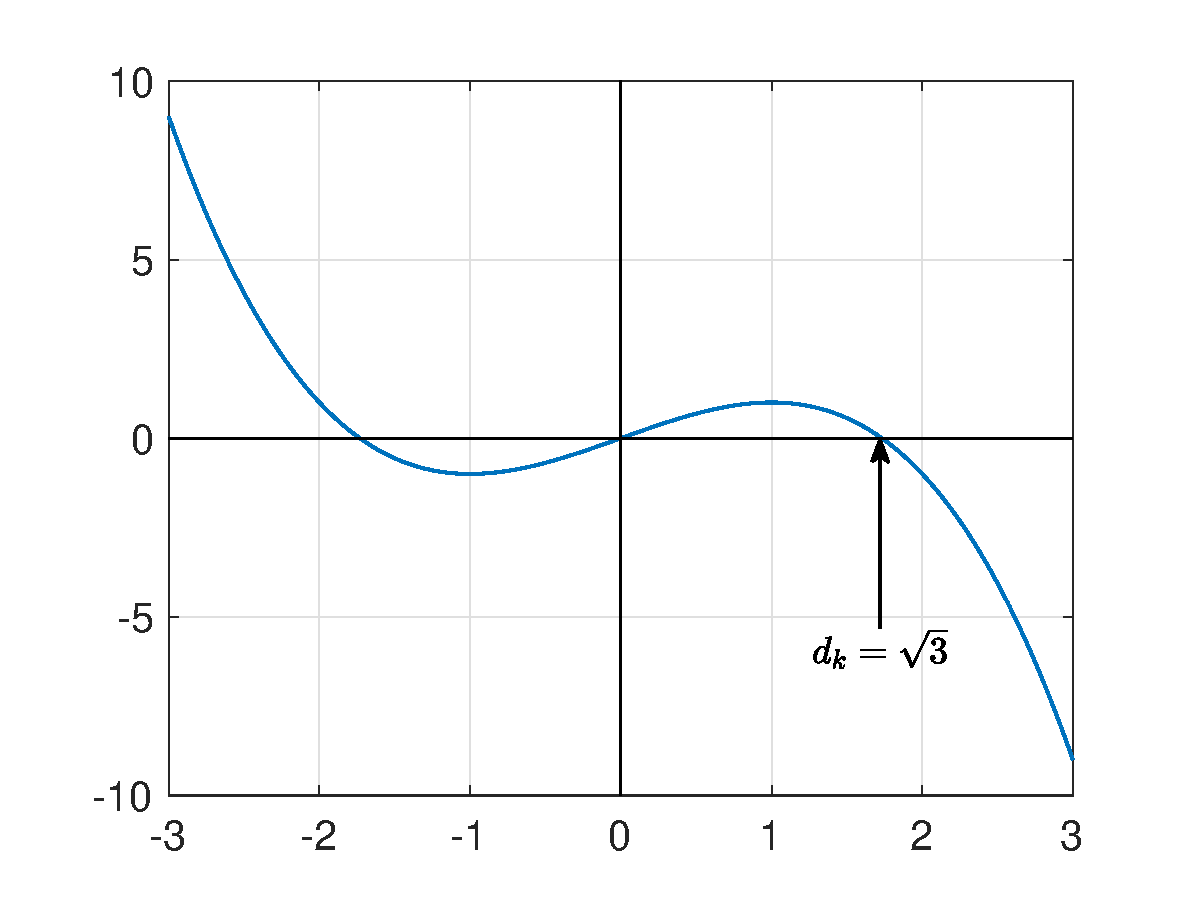
\includegraphics[width=0.5\textwidth]{images/newton-schulz-scalar.eps}
        \caption[The plot of $f(d_k)$ defined in~\eqref{eq:simplified-D-iter}.]{The plot of $f(d_k)$ defined in~\eqref{eq:simplified-D-iter} over $[-3,3]$. Three zeros of $f(d_k)$ are $d_k = -\sqrt{3},0$ and $\sqrt{3}$.}
        \label{fig:11}
    \end{figure}

    Other parts of the real line may still converges to $1$ but the interval of convergence is too short to consider and control (for example, if we start with $d_0 = 2.2$, then $d_1 = f(d_0) = -2.0240$ and $d_2 = 1.1097 \in (0,\sqrt{3})$ which will converges to $1$).

    Remain to show that the convergence is of order $2$. By consider the difference $d_{k+1} - 1$ (similar approach as~\eqref{eq:quadConv}), we have 
    \begin{equation}\label{eq:NS-iter-scalar}
        d_{k+1} - 1 = -\frac 12 (d_k-1)^2 (d_k + 2)
    \end{equation}
    which implies quadratic convergence.
\end{proof}

\begin{theorem}
    [Convergence of the Newton--Schulz iteration~\eqref{eq:ns-iteration}]
    \label{thm:newtonSchulzConverge}
    For $A\in\C\nn$ of rank $n$ which has the polar decomposition $A = UH$, if $\sigma_i(A) \in (0,\sqrt{3})$, then the Newton--Schulz iteration 
    \begin{equation}\notag
        X_{k+1} = \frac 12 X_k(3I-X_k\ctp X_k),\quad X_0 = A,
    \end{equation}
    converges to the unitary factor $U$ quadratically as $k\to\infty$ and 
    \begin{equation}\label{eq:NSconv}
        \gnorm{X_{k+1} - U} \leq \frac 12 \gnorm{X_k + 2U} \gnorm{X_k - U}^2
    \end{equation}
    holds for any unitarily invariant norm.
\end{theorem}

\begin{proof}
    By Lemma~\ref{lemma:scalarNS}, the diagonal entries of $D_k$ converge to $1$ quadratically and this is equivalent as $D_k$ converges to $I$ quadratically as $k\to\infty$. Using the definition of $D_k$, we conclude that $X_k$ converges to $U$, the unitary polar factor of $A$, quadratically.

    From \eqref{eq:NS-iter-scalar} and the proof of Theorem~\ref{thm:newton-converge}, we have 
    \begin{equation}
        \notag 
        \begin{aligned}
            \gnorm{D_{k+1} - I} &= \frac{1}{2}\gnorm{(D_k - I)(D_k - I)(D_k + 2I)} \\
            & \leq \frac{1}{2}\gnorm{D_k - I}^2 \gnorm{D_k + 2I}.\\
            \Rightarrow 
            \gnorm{X_{k+1} - U} &\leq \frac{1}{2} \gnorm{X_k - U}^2 \gnorm{X_k + 2U}.
        \end{aligned}
    \end{equation}
    Hence we proved the quadratic convergence of the Newton-Schulz iteration.
\end{proof}

\section{Operation Count}
In this section, we will evaluate the operation count for one step of Newton's method and one step of the Newton--Schulz iteration. We measure the computational cost by the number of scalar
multiplications, divisions and additions/subtractions. Each of these operations are called a \emph{flop}~\ycite[2002, p.~3]{high:ASNA2}.

\subsection{Operation Count for Newton's Method}
Recall that the Newton's method is 
\begin{equation}
    \notag 
    X_{k+1} = \frac 12(X_k^{-*} + X_k),\quad X_0 = A.
\end{equation}

Each step requires one matrix inversion, one scalar-matrix multiplication and one matrix-matrix addition. The final two operations cost $n^2$ flops respectively. To compute $X_k\inv$, we use the following routine
\begin{enumerate}
    \item Compute the LU decomposition with pivoting $PX_k = LU$, where $P$ is a permutation matrix, $L$ is a lower triangular matrix and $U$ is an upper triangular matrix.
    \item Compute the inverse of $U$ using a sequence of backward substitutions.
    \item Solve the lower triangular system $XL = U\inv$ for $X$.
    \item Compute the inverse $X_k\inv = XP$.
\end{enumerate}

Step 1 requires $2/3n^3 + O(n^2)$ flops, step 2 requires $1/3n^3 + O(n^2)$ flops, step 3 requires $n^3$ flops, and step 4 requires no flops. Therefore, one step of Newton's method requires $2n^3 + O(n^2)$ flops.

\subsection{Operation Count for Newton--Schulz Iteration}
Recall that the Newton--Schulz iteration is 
\begin{equation}\notag
    X_{k+1} = \frac 12 X_k(3I-X_k\ctp X_k),\quad X_0 = A.
\end{equation}
If we rewrite this iteration as
\begin{equation}
    \notag
    X_{k+1} = \frac{3}{2} X_k - \frac{1}{2}X_kX_k\ctp X_k,\quad X_0 = A,
\end{equation}
then clearly, we require two matrix-matrix multiplications and one matrix-matrix subtraction per iteration. Since the latter one requires only $O(n^2)$ flops, the majority of the computational cost will be the matrix level multiplications. Notice that the product $X_k\ctp X_k$ is a symmetric positive definite matrix, hence we can exploit its symmetry during computation. Instead of $2n^3$, we only need 
\begin{equation}
    \notag 
    \sum_{i=1}^n\sum_{j=i}^n\sum_{k=1}^n 2 = n^3 + O(n^2)
\end{equation}
flops to compute $X_k\ctp X_k$. Together with the product $X_k(X_k\ctp X_k)$, the total cost of the Newton--Schulz iteration per step will be $3n^3 + O(n^2)$ flops.

\subsection{Conclusion}
Based on previous discussions, we conclude 
\begin{enumerate}
    \item For Newton's method, which involves matrix inversion, requires $2n^3 + O(n^2)$ flops per step while using the LU decomposition with pivoting.
    \item For Newton--Schulz iteration, which involves matrix multiplications, requires $3n^3 + O(n^2)$ flops per step.
\end{enumerate}

Therefore, ignoring operation counts, the matrix multiplication needs to be 1.5 faster than matrix inversion for Newton--Schulz to be faster than Newton.

\section{Implementation}

In this section, we will present an algorithm that computes the polar decomposition of $A$ using a mixture of the Newton iteration and the Newton--Schulz iteration. The motivation is that matrix multiplication is very fast on high-performance computers. The outline will be the following: Given a nonsingular matrix $A\in\C\nn$, starts with the Newton iteration and switches to the Newton--Schulz iteration when the latter is guaranteed to converge. This procedure will produce the unitary polar factor $U$ of $A$, and then $H$ can be constructed by $H = U\ctp A$. In order to ensure the symmetry for $H$, we calculate $H$ via
\begin{equation}
    \notag 
    H = \frac{1}{2}\left(U\ctp A + A\ctp U\right).
\end{equation}

We need to determine an appropriate condition for us to switch from Newton to Newton--Schulz. From Theorem~\ref{thm:newtonSchulzConverge}, the Newton--Schulz iteration will converge if the input $X_k$ satisfies $\tnorm{X_k} < \sqrt{3}$. However, the matrix 2-norm is rather expensive to compute, and we should view the convergence in the following alternative way.

\begin{theorem}
    \label{thm:Conv-in-R}
    Let $A\in\C\nn$ of rank $n$ has the polar decomposition $A=UH$, and the Newton--Schulz iteration for computing the unitary polar factor $U$ is given by
    \begin{equation}
        \notag 
        X_{k+1} = \frac{1}{2}X_k(3I - X_k\ctp X_k), \quad X_0 = A.
    \end{equation}
    If we define $R_k = I - X_k\ctp X_k$, then $R_k$ satisfies
    \begin{equation}
        \notag
        R_{k+1} = \frac{3}{4}R_k^2 + \frac{1}{4}R_k^3.
    \end{equation}
\end{theorem}

\begin{proof}
    Write $R_{k+1} = I - X_{k+1}\ctp X_{k+1}$, then substitute $X_{k+1} = \frac{3}{2} X_k - \frac{1}{2}X_kX_k\ctp X_k$ into the expression of $R_{k+1}$. The rest are just brute-force substitutions and simplifications, and we will omit the rest.
\end{proof}

We can use $R_{k+1}$ to measure the distance between the iterator $X_k$ and the desired limit $U$ based on the following lemma.

\begin{lemma}
    Let $A\in\C\nn$ have the polar decomposition $A=UH$. Then 
    \begin{equation}
        \label{eq:DistEquiv} 
        \frac{\gnorm{A\ctp A - I}}{1+\sigma_1(A)} \leq \gnorm{A-U} \leq 
        \frac{\gnorm{A\ctp A - I}}{1+\sigma_n(A)},
    \end{equation}
    for any unitarily invariant norm.
\end{lemma}

\begin{proof}
    Let $A$ have the SVD $A=P\Sigma V\ctp$. Then we have two equalities 
    \begin{itemize}
        \item $A\ctp U = U\ctp A$.
        \item $\gnorm{A-U} = \gnorm{\Sigma - I}$.
    \end{itemize}
    Based on the first equality, we can write $A\ctp A - I = (A-U)\ctp (A+U)$, then take a unitarily invariant norm on both sides 
    \begin{equation}
        \notag 
        \begin{aligned}
            \gnorm{A\ctp A - I} &= \gnorm{(A-U)\ctp (A+U)} \\
            & \leq \gnorm{A-U}\tnorm{A+U}\quad \text{\ycite[1991, Cor.~3.5.10]{TopicsInMatrixAnalysis:1991}}\\
            & = (1+\sigma_1(A))\gnorm{A-U},
        \end{aligned}
    \end{equation}
    which gives the lower bound. For the upper bound, we first write $A+U=U(H+I)$, and then we have 
    \begin{equation}
        \notag 
        A\ctp A - I = (A - U)\ctp U(H+I)\quad \Rightarrow \quad (A\ctp A - I)(H + I)\inv = (A-U)\ctp U.
    \end{equation}
    Taking any unitarily invariant norm on both sides, we have 
    \begin{equation}
        \notag
        \begin{aligned}
            \gnorm{(A-U)\ctp U} &= \gnorm{A-U} = \gnorm{(A\ctp A - I)(H + I)\inv}\\
            & \leq \gnorm{A\ctp A - I}\tnorm{(H+I)\inv} \\
            & = \frac{\gnorm{A\ctp A - I}}{1+\sigma_n(A)}.
        \end{aligned}
    \end{equation}
    Hence we proved the inequality~\eqref{eq:DistEquiv}.
\end{proof}

This result shows that the two measures of orthonormality $\gnorm{A\ctp A - I}$ and $\gnorm{A-U}$ are essentially equivalent, hence the residual $\gnorm{X_k\ctp X_k - I}$ of an iterate is essentially the same as the error $\gnorm{U-X_k}$~\ycite[2008, Sec.~8.7]{2008higham-fm}.

\subsection{Switching Condition}
Instead of switching from Newton iteration to Newton--Schulz iteration at the $k$th step where $\tnorm{X_k} < \sqrt{3}$, we can use Theorem~\ref{thm:Conv-in-R} to characterise this absolute convergence. If $\gnorm{R_{k}} < 1$, then 
\begin{equation}
    \notag 
    \gnorm{R_{k+1}} \leq \frac{3}{4}\gnorm{R_k}^2 + \frac{1}{4}\gnorm{R_k}^3 < \frac{3}{4}\gnorm{R_k} + \frac{1}{4}\gnorm{R_k} = \gnorm{R_k},
\end{equation}
which implies that the Newton--Schulz iteration will certainly converge. Therefore, we can compute $R_{k}$ at each step, once $\gnorm{R_k}\leq\theta<1$, we can switch to Newton--Schulz. In~\ycite[1990, p.~652]{hisc90}, it suggests, to ensure fast convergence, $\theta$ should not be too close to $1$ and here we choose $\theta = 0.6$ which is used by \cite{hisc90}.

\subsection{Termination Condition}
Suppose $\eta$ is some positive tolerance, a natural way of terminating an iteration is the following: Define the relative difference $\delta_{k+1} = \gnorm{X_{k+1} - X_{k}}/\gnorm{X_{k+1}}$ between two successive iterators, we stop the iteration once $\delta_{k+1} \leq \eta$. However, as suggested by~\ycite[2008, Sec.~4.9.2]{2008higham-fm}, in floating point arithmetic there is typically no guarantee that $\delta_k$ will reach the tolerance $\eta$. The solution is to add another criterion which terminates the iteration once the relative change has not decreased by a factor of at least 2.

In addition, as suggested by \ycite[2008, p.~208]{2008higham-fm}, $\delta_{k+1}\leq \eta$ tends to terminate the iteration too late. Instead, we can use the following condition:
\begin{equation}
    \notag 
    \gnorm{X_{k+1} - X_{k}}_\infty \le (2\eta)^{1/2}n^{1/2},
\end{equation}
as suggested by \ycite[2008, p.~208]{2008higham-fm} and~\ycite[2003, App.~C]{Kielbasinski2003}.

\subsection{Algorithm}
In summary, the computation of the polar decomposition of $A\in\C\nn$ can be summarized into the Algorithm~\ref{alg:poldec}.

\begin{algorithm}[hbt!]
    \floatname{algorithm}{Algorithm} 
    \caption{Given $A\in\C\nn$ of rank $n$, this algorithm computes the polar decomposition $A = UH$ using both the Newton iteration and the Newton--Schulz iteration. $\eta$ is a positive convergence tolerance which is the machine epsilon at double precision by default.}
    \label{alg:poldec}
    \begin{algorithmic}[1]
        \State Let $X = A$, \inline{switch = false}
        \State tol = $\sqrt{2\eta}\sqrt{n}$, maxiteration = $10^6$
        \For{$i = 1:\text{maxiteration}$} 
            \State {Compute $R_1 = \gnorm{X\ctp X - I}_\infty$}
            \If{$R_k \le 0.6$}
                \State{\inline{switch = true}}
            \EndIf
            \If{\inline{switch}}
                \State{Store $X \to X_{store}$}
                \State{Update $X$ using Newton--Schulz iteration}
                \State{Compute $\delta_{i+1} = \gnorm{X-X_{store}}_\infty/\gnorm{X}_\infty$}
                \State{\itshape \% termination condition}
                \If{$\delta_{i+1} < \text{tol}$ \textbf{OR} ($\delta_{i+1} > \delta_i/2$ \textbf{AND} $i\neq 1$)}
                    \State{\textbf{Break}}
                \EndIf
            \Else 
                \State{Store $X \to X_{store}$}
                \State{Update $X$ using Newton iteration}
                \State{Compute $\delta_{i+1} = \gnorm{X-X_{store}}_\infty$}
            \EndIf
        \EndFor
    \end{algorithmic}
\end{algorithm}

In line 2, we add a \inline{maxiteration} to prevent the algorithm from going forever.
At the beginning of the algorithm, the relative error between successive iteration can have $\delta_{i+1} \approx \delta_i$, which will stop the algorithm immediately. Instead we put the termination condition, line 13--15, inside the Newton--Schulz iteration.
The algorithm can be implemented  using MATLAB as shown in Appendix~\ref{app:poldec.m}.

\section{Numerical Testings}
\subsection{Experiment Setup}
To test the correctness of our code, we examine the relative error $\gnorm{A - UH}_{\infty}/\gnorm{A}_\infty$ and $\gnorm{U\ctp U - I}_\infty$. In addition, I will compare our computed solution $U$ with the reference solution $U_\mathrm{ref}$ which is computed at quadruple precision using Multiprecision Computing Toolbox~\footnote{\url{https://www.advanpix.com/}}.
Our experiments are running under the following environment:
\begin{itemize}
    \item CPU : Intel(R) Core(TM) i5-9600KF CPU @ 3.70GHz
    \item GPU : NVIDIA GeForce RTX 2060
    \item MATLAB Version : 9.12.0.2039608 (R2022a) Update 5
    \item Multiprecision Computing Toolbox : 4.9.0 Build 14753
    \item Random Number Generator : \inline{rng(1)}
\end{itemize}

We will test our MATLAB code in Appendix~\ref{app:poldec.m} using the following matrices:
\begin{itemize}
    \item \inline{randn(n)} : An $\R\nn$ matrix containing pseudorandom values drawn
    from the standard normal distribution. The random number generator is controlled by \inline{rng(1)}.
    \item \inline{eye(8)} : The $8\times 8$ identity matrix.
    \item \inline{hilb(6)} : The $6\times 6$ matrix with elements $1/(i+j-1)$, which is a
    famous example of a badly conditioned matrix.
    \item \inline{magic(6)} : An $6\times 6$ matrix constructed from the integers
    1 through 36 with equal row, column, and diagonal sums.
    \item \inline{hadamard(8)} : A Hadamard matrix of order 8, that is, a matrix $H$
    with elements $+1$ or $-1$ such that $H\ctp H = 8I$.
\end{itemize}

\subsection{Results and Comments}
After applying Algorithm~\ref{alg:poldec} on the above test matrices, we have the data shown in Table~\ref{tab:numerical-data}. The testing routine can be found in Appendix~\ref{app:testingroutine}, and we produce the figures contain how $\gnorm{X_{k+1} - X_{k}}_\infty/\gnorm{X_{k+1}}_\infty$ and $\gnorm{X\ctp X - I}_\infty$ change with respect to the iteration. The figures (except for \inline{eye(8)}) can be found in Appendix~\ref{app:figs}. We have the following comments on the results:

\begin{itemize}
    \item \inline{randn(n)}: The algorithm works perfectly, and we indeed have a polar decomposition $A = UH$, and the unitary polar factor is unitary as expected. 
    \item \inline{eye(8)}: The algorithm converges after one iteration since the input $A$ is the same as the expected result $U$, which are both $I_8$. The polar decomposition for $I_8$ is then $I_8 \cdot I_8$.
    \item \inline{hilb(6)}: Hilbert matrix is badly conditioned as seen from the Table~\ref{tab:numerical-data}, $\kappa_\infty(H_6)$ is $O(10^7)$. Due to bad conditioning, although $\inorm{H\ctp H - I}$ can be small, but after one iteration, the matrix $X_{1} = (H^{-*} + H)/2$ can have a large $\inorm{X_1\ctp X_1 - I}$ as shown in Figure~\ref{fig:hilb6} and the following output.
\begin{lstlisting}
>> rng(1); H = hilb(6); norm(H'*H-eye(6),inf)
ans =
   3.1932e+00
>> X = 0.5*(inv(H)'+H); norm(X'*X-eye(6),inf)
ans =
   2.7423e+13
\end{lstlisting}
Therefore, the Newton's method requires a lot of iterations in order to drag the quantity $\inorm{X_k\ctp X_k - I}$ back to $0.6$.
    \item \inline{magic(6)}: The magic square is a singular matrix, and therefore our algorithm is not applicable. Nevertheless, we can run our code on this matrix anyway. Notice that the quantity $\inorm{A-UH}/\inorm{A}$ is large compared to the machine epsilon of double precision because $A$ is a badly conditioned matrix. The computed $H$ is positive semidefinite as expected from Definition~\ref{def:pol-dec-definition}. 
    \item \inline{hadamard(8)}: The Hadamard matrix of order 8 is well conditioned, and the result is perfect. Since the input Hadamard matrix $A$ has the property that $A\ctp A = 8I_8$, therefore by Theorem~\ref{def:pol-dec-definition}, the positive definite part has the form $H = (A\ctp A)^{1/2} = \sqrt{8}I \approx 2.8284I_8$. The computed result indeed satisfies this structure with $$\inorm{H_\mathrm{comp} - H_\mathrm{expect}}\approx 8.8818\times 10^{-16}.$$ 
\end{itemize}
\begin{table}[H]
    \centering 
    \caption{Results for applying \inline{poldec.m} in Appendix~\ref{app:poldec.m} to the test matrices.}
    \label{tab:numerical-data}
    \begin{tabular}{lccccc}
        \toprule 
            {Matrix $A$} & {\(\displaystyle \kappa_\infty(A)\)} & {Iteration} & {\(\displaystyle \frac{\gnorm{A - UH}_\infty}{\gnorm{A}_\infty}\)} & {\(\displaystyle \gnorm{U\ctp U - I}_{\infty}\)} & {$\gnorm{U - U_{\mathrm{ref}}}_{\infty}$}\\
        \toprule 
        \texttt{randn(20)} & 1.6827e+03 & 8 & 3.1315e-16 & 4.6783e-16 & 5.6639e-16 \\
        \midrule 
        \texttt{randn(50)} & 1.0280e+03 & 9 & 6.8817e-16 & 8.3942e-16 & 1.5430e-15\\
        \midrule 
        \texttt{randn(100)} & 2.1124e+03 & 9 & 1.1056e-15 & 1.1314e-15 & 2.3256e-15\\
        \midrule 
        \texttt{eye(8)} & 1 & 1 & 0 & 0 & 0\\
        \midrule 
        \texttt{hilb(6)} & 2.9070e+07 & 28 & 1.3028e-16 & 2.2303e-16 & 1.1334e-16  \\
        \midrule 
        \texttt{magic(6)} & 9.9980e+17 & 58 & 4.4338e-03 & 4.2653e-16 & 3.3307e-16\\
        \midrule 
        \texttt{hadamard(8)} & 8 & 7 & 2.4980e-16 & 3.0175e-16 & 3.8858e-16\\
        \bottomrule
    \end{tabular}
\end{table}

\section{Further Application}
We can utilize the polar decomposition to compute the square root of a symmetric positive definite matrix. Given a symmetric positive definite matrix $A\in\R\nn$, we can firstly compute the Cholesky factor $R$ of $A$ such that $A = R\tp R$, and then apply Algorithm~\ref{alg:poldec} to $R$ which gives $R = UH$ where $U$ is unitary (in this case, orthogonal) and $H$ is symmetric positive definite. Substitute back into the Cholesky decomposition of $A$, we have 
\begin{equation}
    \notag 
    A = R\tp R = (UH)\tp (UH) = H\tp U\tp U H = H^2.
\end{equation}
Therefore, the symmetric positive definite part of the polar decomposition of the Cholesky factor of $A$ is the square root of $A$ for any symmetric positive definite matrix $A$.

The implementation is straightforward using MATLAB builtin function \inline{chol} which computes the Cholesky factor, and the function \inline{polsqrt.m} can be found in Appendix~\ref{app:matrix-squareroot}. A simple test is carried out below:
\begin{lstlisting}
>> rng(1); A = gallery('randsvd',50,-100); 
>> H = polsqrt(A); disp(norm(H*H - A));
    2.9638e-16
\end{lstlisting}
The result shows that our code is valid. Here \inline{gallery('randsvd',50,-100)} generates a symmetric positive definite matrix $A\in\R^{50\times 50}$ with fixed condition number $100$.




\newpage 
\bibliographystyle{pre/nj-plain}
\bibliography{pre/bib}
\newpage 

\appendix
\section{Code for Algorithm~\ref{alg:poldec}} \label{app:poldec.m}
\begin{lstlisting}
function [X, H, its, delta, Rk] = poldec(A, TOL)
%POLDEC Polar decomposition.
% [U, H, ITS, DELTA, RK] = poldec(A) computes the polar decomposition 
% A = U*H of the square, nonsingular matrix A. ITS is the number of
% iterations for convergence. DELTA is the relative error between 
% successive iterations. RK is the norm(X'X - I) at each iteration.
[n,m] = size(A);
if n ~= m
    error('Input matrix is not square!');
end
if nargin == 2
    err = TOL;
else
    err = eps("double");
end
I = eye(n); term_tol = sqrt(2*err)*sqrt(n); maxiter = 1e6;
X = A; switched = false; 
delta = zeros(maxiter,1); Rk = zeros(maxiter,1);
for its = 1:maxiter
    % check if switch to Newton Schulz
    Rk(its) = norm(X'*X - I,inf);
    if Rk(its) <= 0.6
        switched = true;
    end
    % apply appropriate iterations
    if switched % Newton Schulz iteration
        tmp = X;
        X = 1.5*X - 0.5*X*(X'*X);
        delta(its+1) = norm(X - tmp,inf)/norm(X,inf); % store error
        % termination condition
        if delta(its+1) < term_tol || (delta(its+1) > delta(its)/(2) && its ~= 1)
            break;
        end
    else % Newton iteration
        tmp = X;
        X = 0.5*(inv(X)' + X);
        delta(its+1) = norm(X - tmp,inf)/norm(X,inf); % store error
    end
end
H = 0.5*(X'*A + A'*X); % construct H
end
\end{lstlisting}
\newpage 
\section{Testing Routine} \label{app:testingroutine}
\begin{lstlisting}
% testing routine
clc; clear; close all; format short e
rng(1);
print = true;
A = hadamard(8); A_mp = mp(A, 34);
term_tol = sqrt(2*eps("double"))*sqrt(size(A,1));
[U_d,H_d,its_d,del_d,Rk_d] = poldec(A);
[U_q,H_q,its_q,del_q,Rk_q] = poldec(A,5e-34);
% printing results
fprintf("Condition number = %.4d\n", cond(A,inf));
fprintf("Iteration required = %d\n", its_d);
tmp1 = norm(A - U_d*H_d, inf)/norm(A,inf);
fprintf("norm(A-UH)/norm(A) = %.4d\n", tmp1);
tmp2 = norm(U_d'*U_d - eye(size(A,1)));
fprintf("norm(U'*U-I) = %.4d\n", tmp2);
tmp3 = norm(U_d - U_q,inf);
fprintf("norm(U-U_ref) = %.4d\n", tmp3);

if print 
    figure('Renderer', 'painters', 'Position', [200 200 900 900])
    semilogy(1:its_d, del_d(2:its_d+1),'-^k', 'LineWidth', 2);
    hold on;
    semilogy(1:its_d, Rk_d(1:its_d),'-^r', 'LineWidth', 2);
    semilogy(1:its_d, ones(1,its_d).*term_tol, '--b', 'LineWidth', 2);
    legend("$\|X_{k+1}-X_{k}\|_{\infty}/\|X_{k+1}\|_{\infty}$", ...
        "$\|X_k^*X_k - I\|_{\infty}$", ...
        "Terminate tolerance", ...
        "Location","southwest", ...
        "Interpreter", "latex");
    xlabel("Iteration");
    axis square;
    set(gca, "FontSize", 30)    
end
\end{lstlisting}

\section{Routine for Matrix Square Root}\label{app:matrix-squareroot}
\begin{lstlisting}
function H = polsqrt(A)
%POLSQRT Matrix square root using polar decomposition.
% H = poldec(A) computes the matrix square root of the symmetric 
% positive definite matrix A, such that norm(H^2 - A) is small.
R = chol(A);
[~,H] = poldec(R);
end
\end{lstlisting}

\section{Figures}\label{app:figs}

\begin{figure}[H]
    \centering
    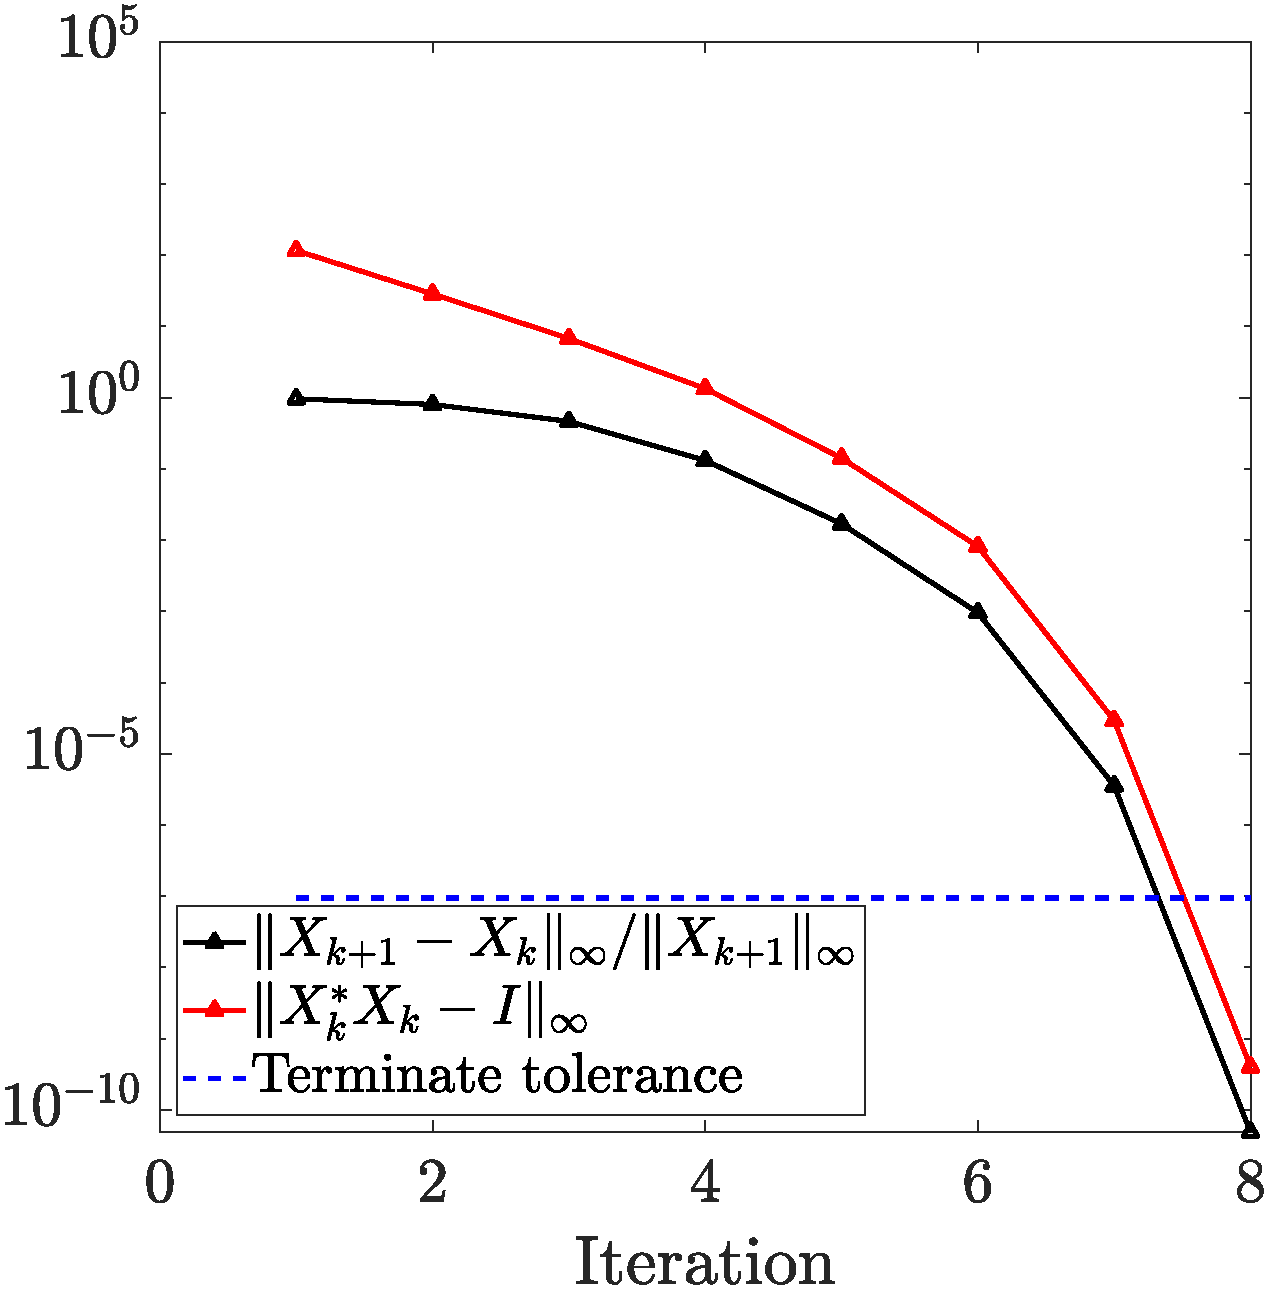
\includegraphics[width=0.59\textwidth]{../code/randn20.pdf}
    \caption{Behaviour of $\gnorm{X_{k+1} - X_{k}}_\infty/\gnorm{X_{k+1}}_\infty$ and $\gnorm{X\ctp X - I}_\infty$ with respect to the iteration when applying \inline{poldec} on \inline{randn(20)}.}
\end{figure}

\begin{figure}[H]
    \centering
    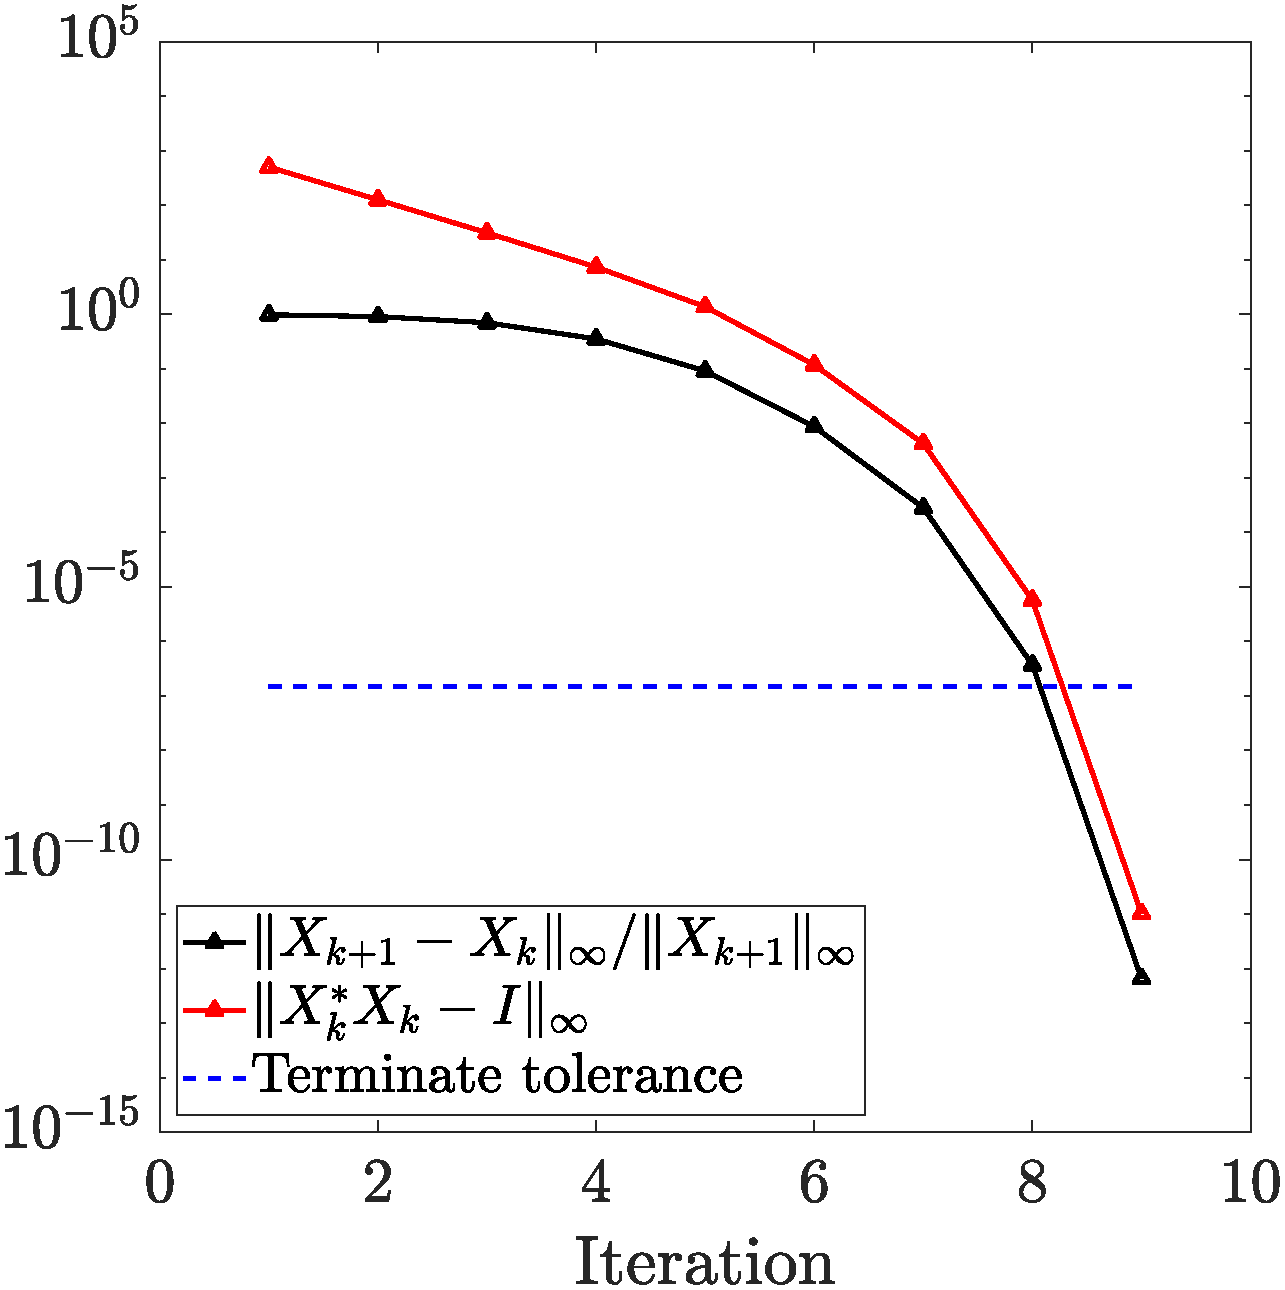
\includegraphics[width=0.6\textwidth]{../code/randn50.pdf}
    \caption{Behaviour of $\gnorm{X_{k+1} - X_{k}}_\infty/\gnorm{X_{k+1}}_\infty$ and $\gnorm{X\ctp X - I}_\infty$ with respect to the iteration when applying \inline{poldec} on \inline{randn(50)}.}
\end{figure}

\begin{figure}[H]
    \centering
    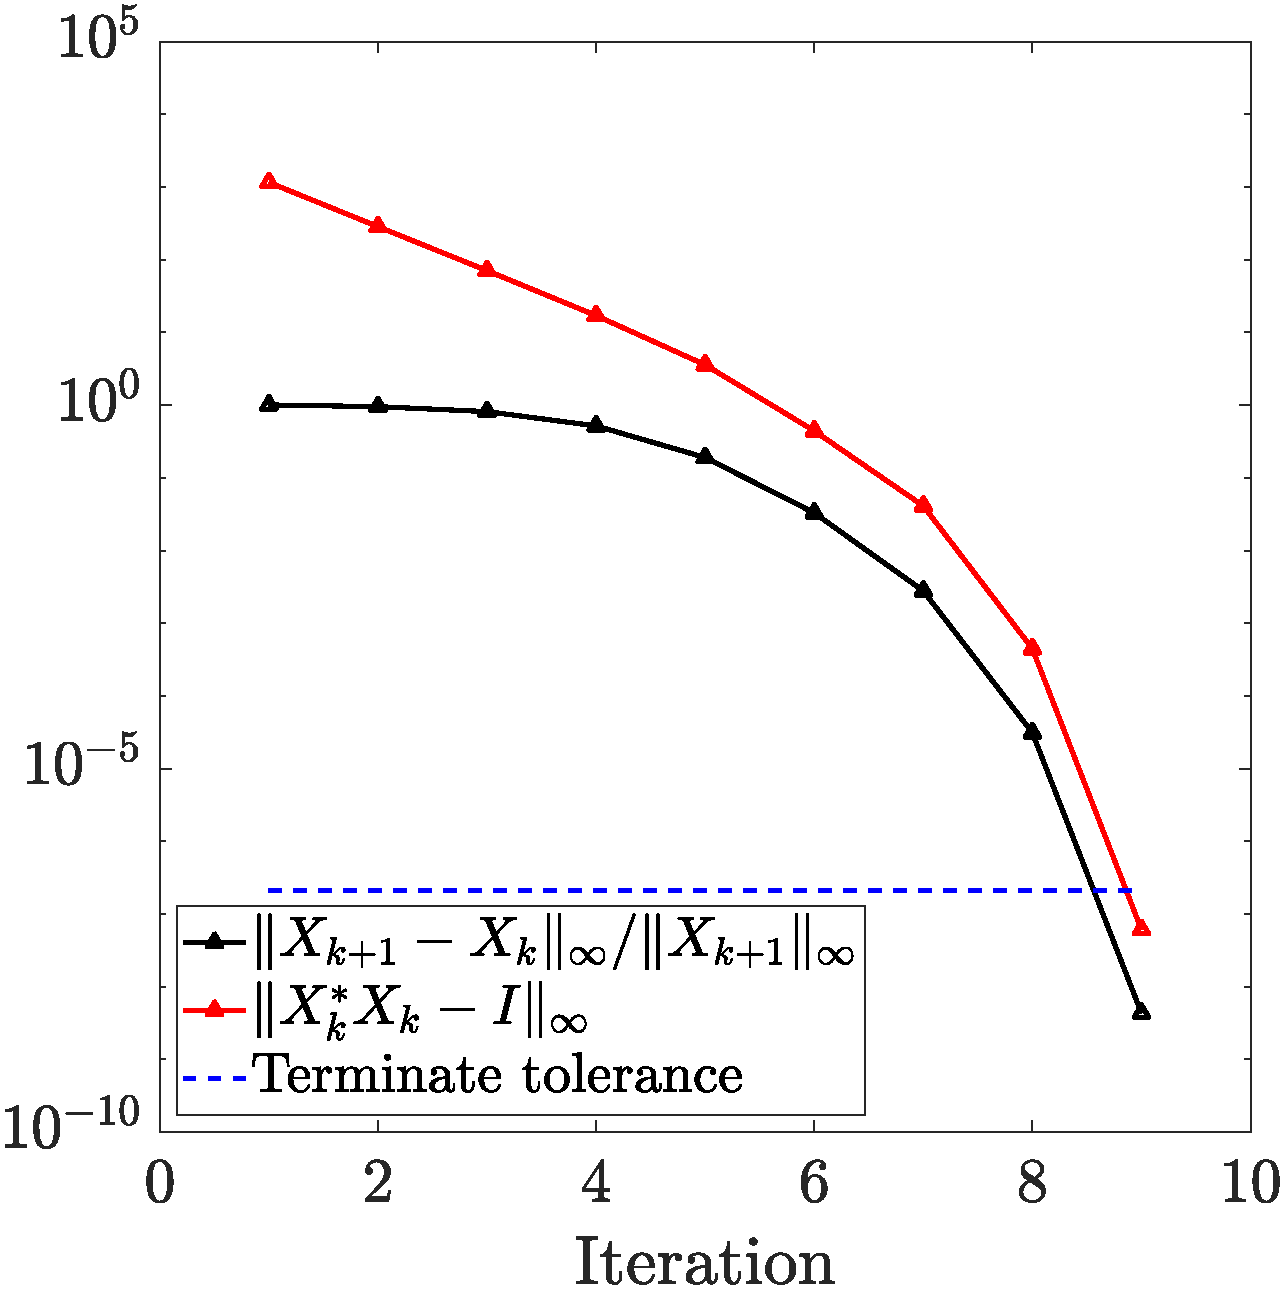
\includegraphics[width=0.6\textwidth]{../code/randn100.pdf}
    \caption{Behaviour of $\gnorm{X_{k+1} - X_{k}}_\infty/\gnorm{X_{k+1}}_\infty$ and $\gnorm{X\ctp X - I}_\infty$ with respect to the iteration when applying \inline{poldec} on \inline{randn(100)}.}
\end{figure}

\begin{figure}[H]
    \centering
    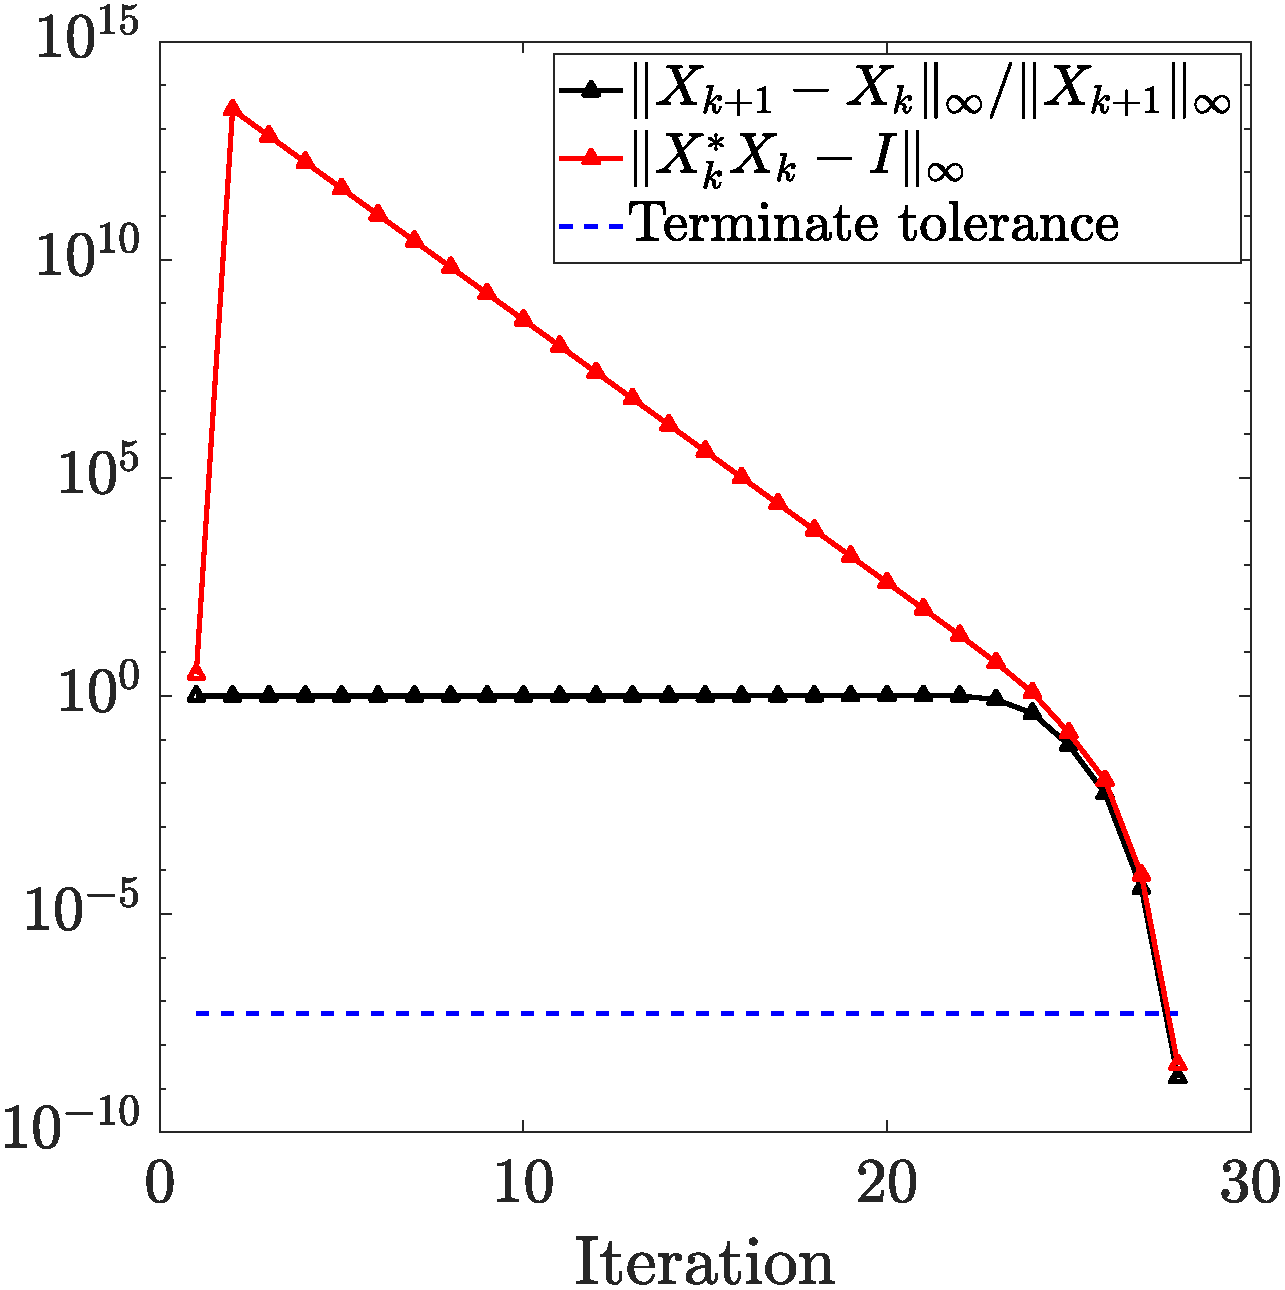
\includegraphics[width=0.6\textwidth]{../code/hilb6.pdf}
    \caption{Behaviour of $\gnorm{X_{k+1} - X_{k}}_\infty/\gnorm{X_{k+1}}_\infty$ and $\gnorm{X\ctp X - I}_\infty$ with respect to the iteration when applying \inline{poldec} on \inline{hilb(6)}.}
    \label{fig:hilb6}
\end{figure}

\begin{figure}[H]
    \centering
    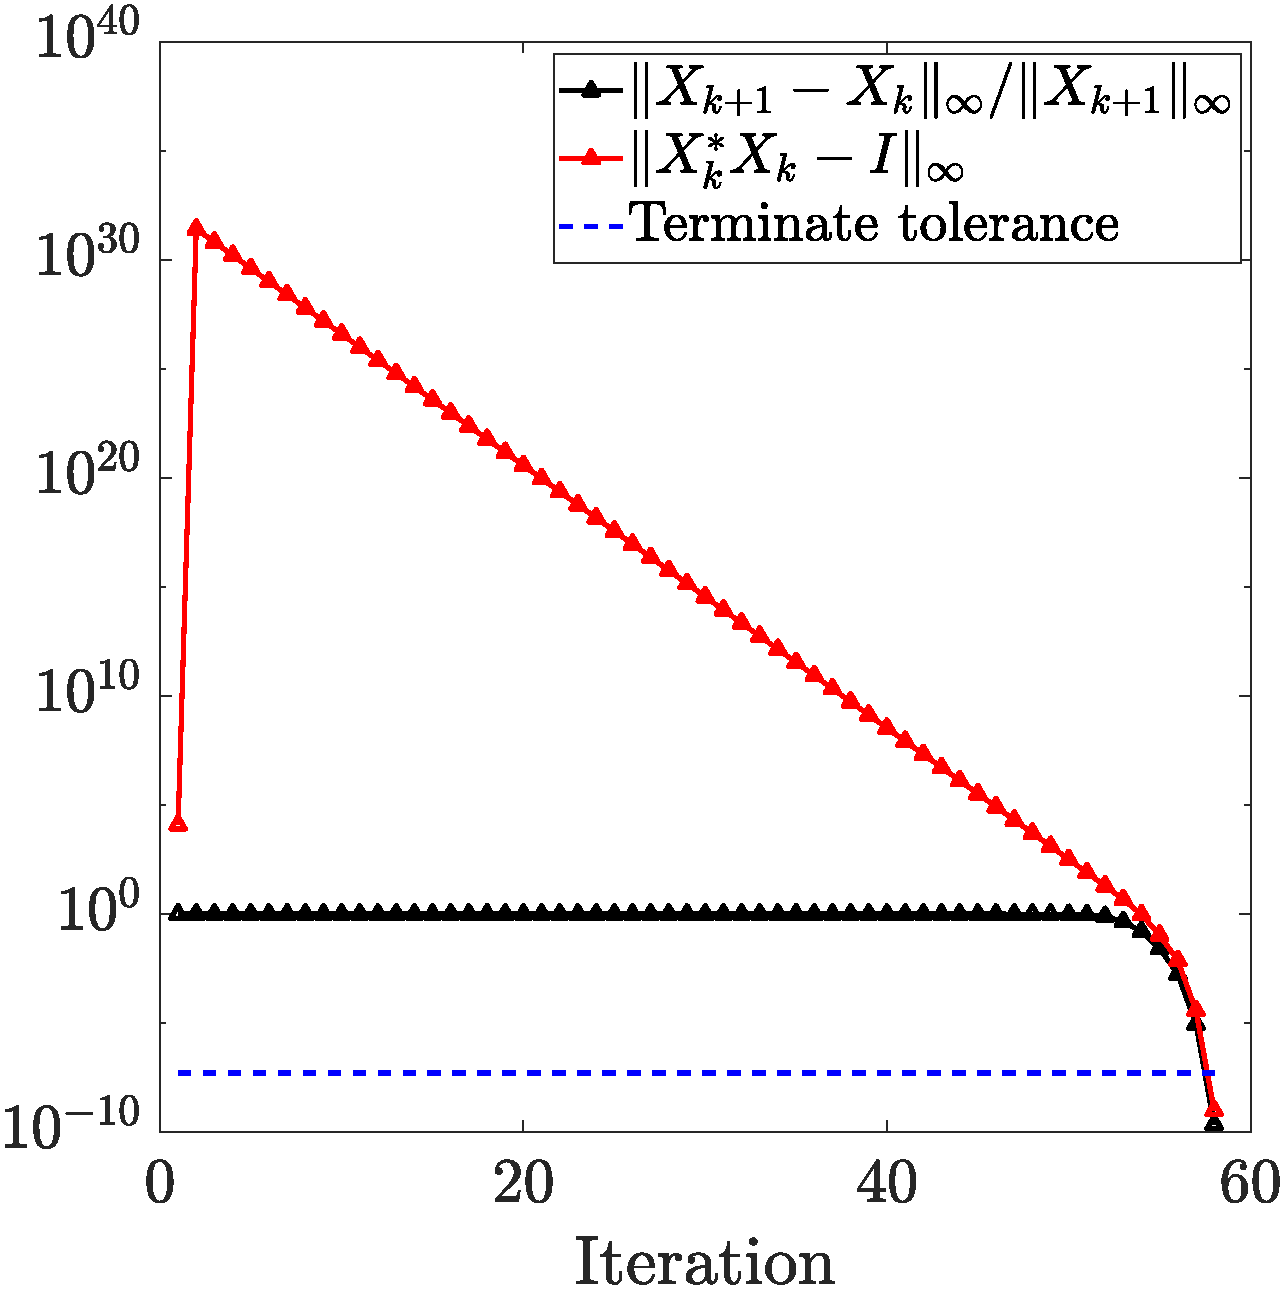
\includegraphics[width=0.6\textwidth]{../code/magic6.pdf}
    \caption{Behaviour of $\gnorm{X_{k+1} - X_{k}}_\infty/\gnorm{X_{k+1}}_\infty$ and $\gnorm{X\ctp X - I}_\infty$ with respect to the iteration when applying \inline{poldec} on \inline{magic(6)}.}
\end{figure}

\begin{figure}[H]
    \centering
    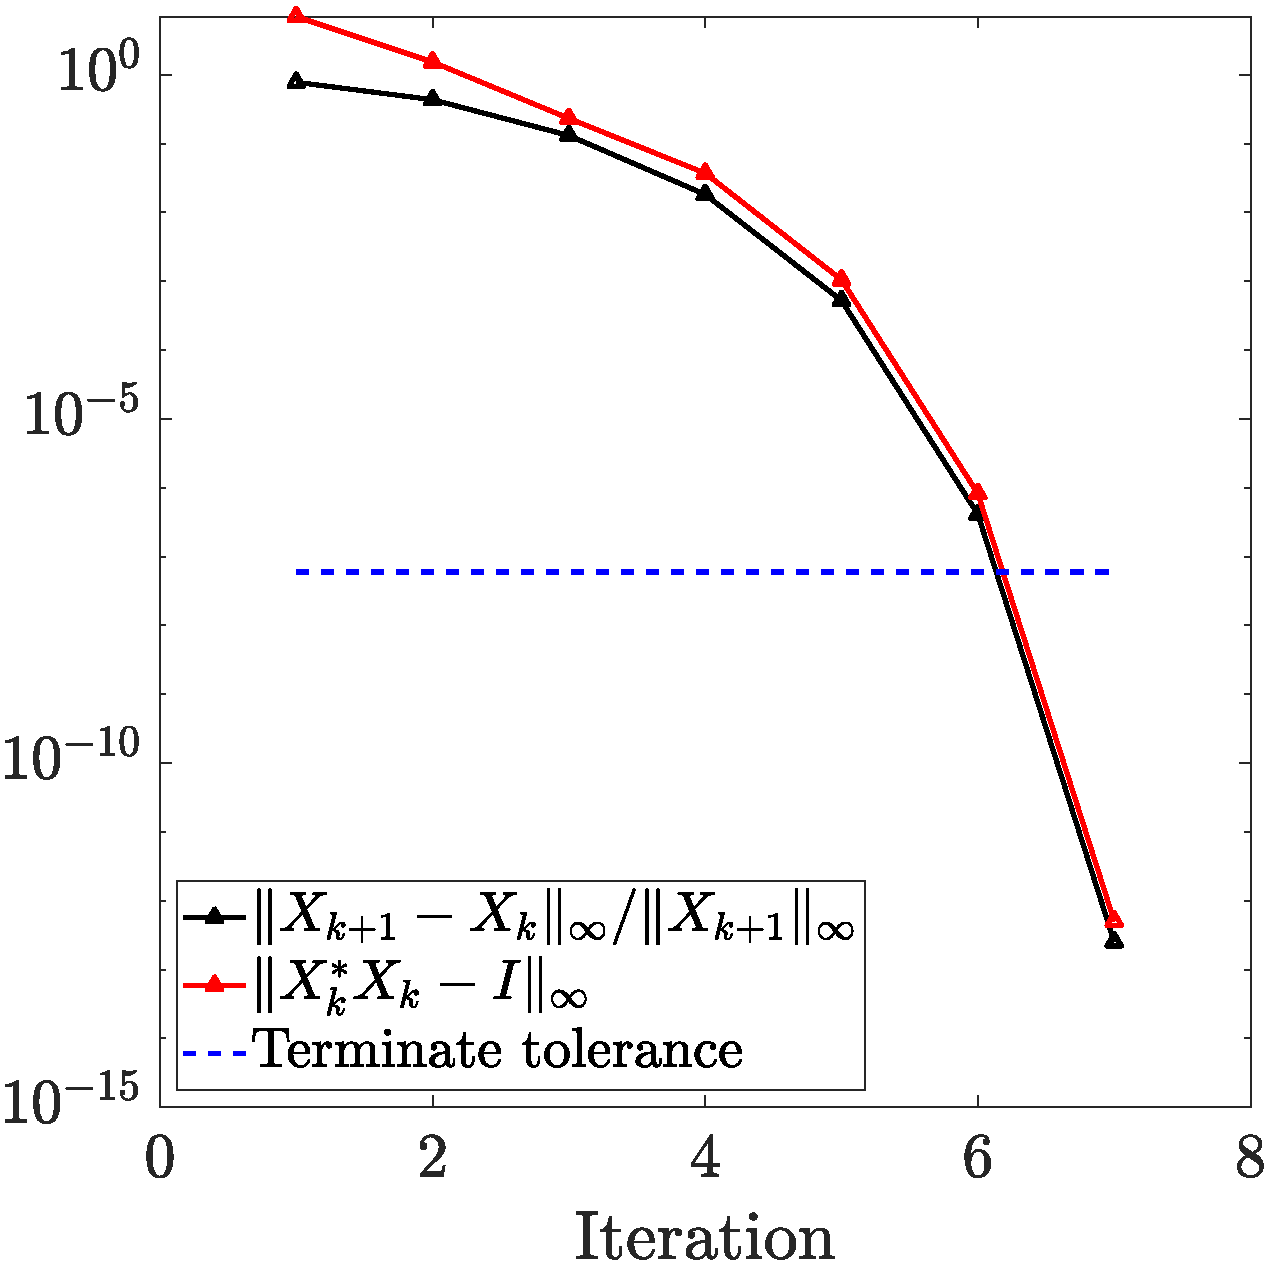
\includegraphics[width=0.6\textwidth]{../code/hadamard8.pdf}
    \caption{Behaviour of $\gnorm{X_{k+1} - X_{k}}_\infty/\gnorm{X_{k+1}}_\infty$ and $\gnorm{X\ctp X - I}_\infty$ with respect to the iteration when applying \inline{poldec} on \inline{hadamard(8)}.}
\end{figure}

\end{document}
